\documentclass[a4paper,10pt]{ctexart}
\usepackage{graphicx}
\usepackage{float}%用于正确的安放图片的位置
\usepackage{geometry}
\usepackage{color}%用于设置字体的颜色 用法:{\color{red}{I love you}}
\geometry{margin=1cm}
\begin{document}
\pagestyle{empty}

\begin{center}
\Huge\textbf{MPTCP~~源~~码~~分~~析}
\end{center}

\tableofcontents

\section{前言}
这篇文章是从博客上面看到的,感觉对我们还是挺重要的,于是把它整理成文档,方便我们学习。网址如下:\\
\verb|http://www.cnblogs.com/lxgeek/p/4187164.html|\\
(在网页上观看的效果更好)从MPTCP的理解开始,一篇接着一篇一直把源码分析读完,很关键。

{\color{red}{说明:红色部分是我添加的注解}}

\section{MPTCP综述}
\subsection{背景}
随着技术的发展许多设备具有了多个网络接口,而TCP依然是一个单线路的协议,在TCP的通信过程中发端和收端都不能随意变换地址。我们可以利用多个网络接口的这一特性来改善性能和有效冗余。例如:你的手机同时连接WIFI信号和3G信号的时候(注意:这两个接口都是使用IP地址的,所以可以使用MPTCP,如果是蓝牙,没有IP地址,就不能使用MPTCP),如果WIFI关掉,使用WIFI进行的TCP连接就会断开,而不能有效利用3G网络继续收发数据。这里的问题还有一个很重要的意义就是在移动的网络中,需要切换地址的网络中有很重要的作用,清华现在正在做高铁上的MPTCP相关研究。MPTCP可以解决这些问题。

\subsection{简介}
MPTCP允许在一条TCP链路中建立多个子通道。当一条通道按照三次握手的方式建立起来后,可以按照三次握手的方式建立其他的子通道,这些通道以三次握手建立连接和四次握手解除连接。这些通道都会绑定于MPTCP session,发送端的数据可以选择其中一条通道进行传输。

\subsection{MPTCP设计原则}
MPTCP的设计遵守以下两个原则:
\begin{itemize}
	\item 应用程序的兼容性,应用程序只要可以运行在TCP环境下,就可以在没有任何修改的情况下,运行于MPTCP环境。{\color{red}{可能应用程序也需要进行MPTCP改造}}
	\item 网络的兼容性,MPTCP兼容其他协议。{\color{red}{我覺得MPTCP就是给TCP加了一层,所以所谓的兼容其他的协议,只是兼容TCP而已,因为它只使用TCP子流}}
\end{itemize}

\subsection{在协议栈中的位置}
在协议栈中的位置可以用图~\ref{label:MPTCP在协议栈中的位置}表示。
\begin{figure}[H]
	\centering
	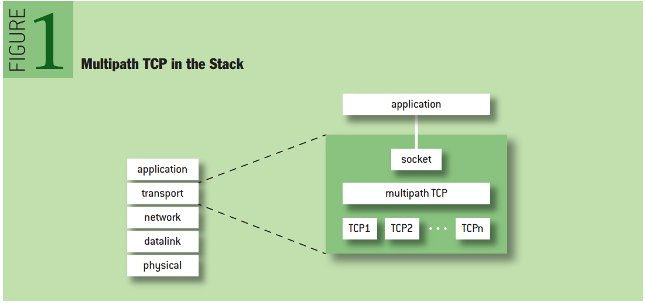
\includegraphics[width=10cm]{dias/MPTCP_position_in_protocol_stack.jpg}
	\caption{MPTCP在协议栈中的位置}
	\label{label:MPTCP在协议栈中的位置}
\end{figure}
在图中我们可以看到,其实MPTCP这一层算是重新搞出的一层,很明显增加了网络的复杂性,这必然会导致效率降低,如果它带来的提升不足以弥补这些负面效应,那也是没有意义的。具体怎么样,看看MPTCP1.0做得如何。
\newpage
\section{建立连接过程}
\subsection{简述建立连接过程}
MPTCP依然按照正常的TCP进行三次握手,只是在握手过程中增加了MPTCP特有的信息,三次握手过程如下图~\ref{label:建立连接过程}:
\begin{figure}[H]
  \centering
  % Requires \usepackage{graphicx}
  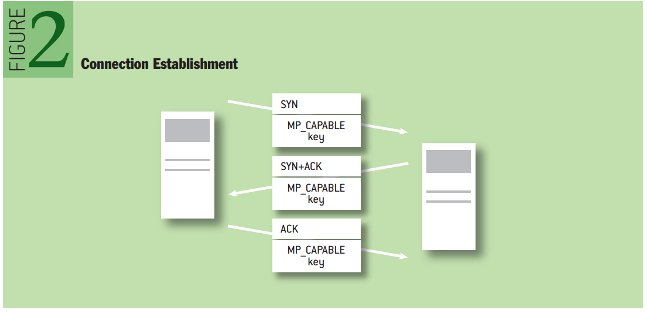
\includegraphics[width=10cm]{dias/Connection_Establishment.jpg}\\
  \caption{建立连接过程}
  \label{label:建立连接过程}
\end{figure}
左边客户端发送的第一个SYN包携带有客户端自身的KEY,右边发送SYN/ACK的时候携带了自身的KEY,而最后左边的客户端发送最后一个ACK的时候携带着双方的KEY。MPTCP中关于MP\_CAPABLE的定义如图~\ref{label:MPCAPABLE的定义}:
\begin{figure}[H]
  \centering
  % Requires \usepackage{graphicx}
  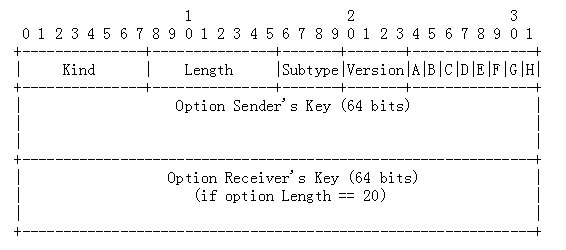
\includegraphics[width=10cm]{dias/Definition_of_MP_CAPABLE.jpg}\\
  \caption{MP\_CAPABLE的定义}
  \label{label:MPCAPABLE的定义}
\end{figure}

\begin{figure}[H]
  \centering
  % Requires \usepackage{graphicx}
  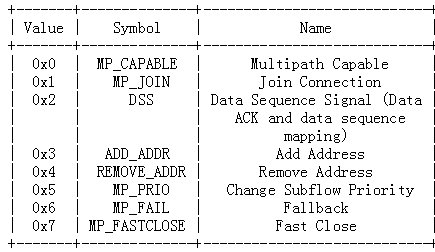
\includegraphics[width=10cm]{dias/Definition_of_Subtype.jpg}\\
  \caption{Subtype的定义}
  \label{fig:Subtype的定义}
\end{figure}

\subsection{建立连接过程的内核实现}
MPTCP在客户端上发送SYN包的调用情况如下:
\begin{figure}[H]
  \centering
  % Requires \usepackage{graphicx}
  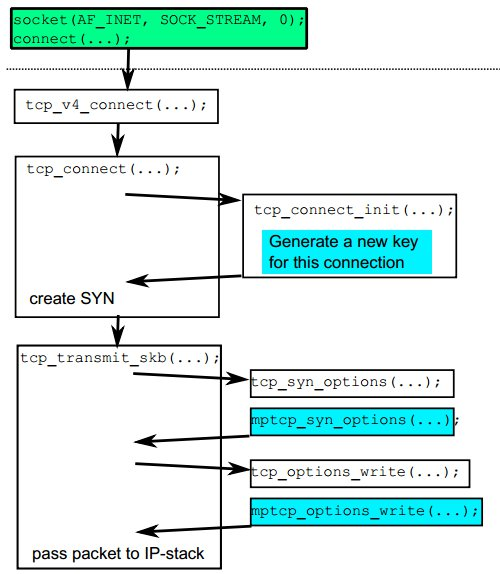
\includegraphics[width=10cm]{dias/Invoke_SYN_in_Cilent.jpg}\\
  \caption{客户端上发送SYN包的调用情况}
\end{figure}
关键函数为mptcp\_syn\_options对MPTCP选项的填充,源码如下:
\small\begin{verbatim}
"net/mptcp/mptcp_output.c" line 843 of 1667
843 void mptcp_syn_options(struct sock *sk, struct tcp_out_options *opts,unsigned *remaining)
845 {
846     struct tcp_sock *tp = tcp_sk(sk);
847
848     opts->options |= OPTION_MPTCP;
849     if (is_master_tp(tp)) {
850         opts->mptcp_options |= OPTION_MP_CAPABLE | OPTION_TYPE_SYN;
851         *remaining -= MPTCP_SUB_LEN_CAPABLE_SYN_ALIGN;
852         opts->mp_capable.sender_key = tp->mptcp_loc_key;
853         opts->dss_csum = !!sysctl_mptcp_checksum;
854     } else {
855         struct mptcp_cb *mpcb = tp->mpcb;
856
857         opts->mptcp_options |= OPTION_MP_JOIN | OPTION_TYPE_SYN;
858         *remaining -= MPTCP_SUB_LEN_JOIN_SYN_ALIGN;
859         opts->mp_join_syns.token = mpcb->mptcp_rem_token;
860         opts->mp_join_syns.low_prio  = tp->mptcp->low_prio;
861         opts->addr_id = tp->mptcp->loc_id;
862         opts->mp_join_syns.sender_nonce = tp->mptcp->mptcp_loc_nonce;
863     }
864 }
\end{verbatim}\normalsize
由于三次握手的肯定是master sock,在850行到853行对MPTCP选项进行了赋值。相应的服务端发送SYN/ACK包时使用mptcp\_synack\_options 函数对选项进行了赋值。而最后一个ACK包则是调用函数mptcp\_established\_options操作。
\subsection{结论}
\begin{itemize}
  \item MPTCP利用TCP的三次握手进行了KEY信息的交换。
\end{itemize}
\newpage
\section{建立子路径}
\subsection{简述建立子路径}
MPTCP在进行三次握手之后,客户端和服务端会进行地址信息的交换,让对方知道彼此未用的地址信息。当客户端知道服务端的地址后就可以建立其他子路径。三次握手和建立子路径的过程如下图:
\begin{figure}[H]
  \centering
  % Requires \usepackage{graphicx}
  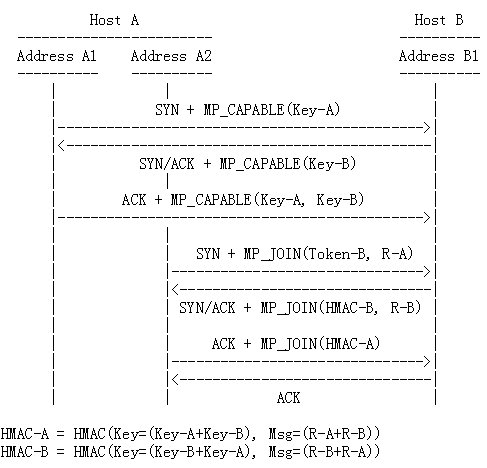
\includegraphics[width=8cm]{dias/Create_Subflows.jpg}\\
  \caption{建立子路径}
\end{figure}

关于Token、随机数R、以及HMAC(Hash-based Message Authentication Code)的详细解释可以阅读参考:\verb|https://tools.ietf.org/html/rfc6824#section-3.2|。

\subsection{建立子路径的内核实现}
这里我们主要关注建立子路径过程中,master sock对slave sock的影响。当客户端发送第一个SYN准备建立子路径的时候就会调用mptcp\_init4\_subsockets来创建一个新的socket和相应的sock。
\small\begin{verbatim}
"net/mptcp/mptcp_ipv4.c" line 328 of 488
328 int mptcp_init4_subsockets(struct sock *meta_sk, const struct mptcp_loc4 *loc,
329                struct mptcp_rem4 *rem)
330 {
331     struct tcp_sock *tp;
332     struct sock *sk;
333     struct sockaddr_in loc_in, rem_in;
334     struct socket sock;
335     int ulid_size = 0, ret;
336
337     /** First, create and prepare the new socket */
338
339     sock.type = meta_sk->sk_socket->type;
340     sock.state = SS_UNCONNECTED;
341     sock.wq = meta_sk->sk_socket->wq;
342     sock.file = meta_sk->sk_socket->file;
343     sock.ops = NULL;
344
345     ret = inet_create(sock_net(meta_sk), &sock, IPPROTO_TCP, 1);
346     if (unlikely(ret < 0)) {
347         mptcp_debug("%s inet_create failed ret: %d\n", __func__, ret);
348         return ret;
349     }
350
351     sk = sock.sk;
352     tp = tcp_sk(sk);
\end{verbatim}\normalsize
第345行的函数inet\_create创建了子路径的socket和sock。
\small\begin{verbatim}
354     /* All subsockets need the MPTCP-lock-class */
355     lockdep_set_class_and_name(&(sk)->sk_lock.slock, &meta_slock_key, "slock-AF_INET-MPTCP");
356     lockdep_init_map(&(sk)->sk_lock.dep_map, "sk_lock-AF_INET-MPTCP", &meta_key, 0);
357
358     if (mptcp_add_sock(meta_sk, sk, loc->loc4_id, rem->rem4_id, GFP_KERNEL))
359         goto error;
360
361     tp->mptcp->slave_sk = 1;
362     tp->mptcp->low_prio = loc->low_prio;
363
364     /* Initializing the timer for an MPTCP subflow */
365     setup_timer(&tp->mptcp->mptcp_ack_timer, mptcp_ack_handler, (unsigned long)sk);
\end{verbatim}\normalsize
第358行的mptcp\_add\_sock将master sock 和 子路径的sock联系起来。第361行表面此sock为 slave subsock。\\
第362行设置此子路径是否为备用路径。只有现在路径都不可用的情况下,才会通过备用子路径发送数据。\\
第365行设置的定时器用于重发建立子路径的最后一个ACK,这样做是为了保证上图中的HMAC-A可以送达。
\small\begin{verbatim}
369     ulid_size = sizeof(struct sockaddr_in);
370     loc_in.sin_family = AF_INET;
371     rem_in.sin_family = AF_INET;
372     loc_in.sin_port = 0;
373     if (rem->port)
374         rem_in.sin_port = rem->port;
375     else
376         rem_in.sin_port = inet_sk(meta_sk)->inet_dport;
377     loc_in.sin_addr = loc->addr;
378     rem_in.sin_addr = rem->addr;
379
380     ret = sock.ops->bind(&sock, (struct sockaddr *)&loc_in, ulid_size);
381     if (ret < 0) {
382         mptcp_debug("%s: MPTCP subsocket bind() failed, error %d\n",
383                 __func__, ret);
384         goto error;
385     }
386
387     mptcp_debug("%s: token %#x pi %d src_addr:%pI4:%d dst_addr:%pI4:%d\n",
388             __func__, tcp_sk(meta_sk)->mpcb->mptcp_loc_token,
389             tp->mptcp->path_index, &loc_in.sin_addr,
390             ntohs(loc_in.sin_port), &rem_in.sin_addr,
391             ntohs(rem_in.sin_port));
392
393     if (tcp_sk(meta_sk)->mpcb->pm_ops->init_subsocket_v4)
394         tcp_sk(meta_sk)->mpcb->pm_ops->init_subsocket_v4(sk, rem->addr);
395
396     ret = sock.ops->connect(&sock, (struct sockaddr *)&rem_in,
397                 ulid_size, O_NONBLOCK);
398     if (ret < 0 && ret != -EINPROGRESS) {
399         mptcp_debug("%s: MPTCP subsocket connect() failed, error %d\n",
400                 __func__, ret);
401         goto error;
402     }
\end{verbatim}\normalsize
第380行是将子路径的socket的与地址绑定。第396行此套接字将会调用tcp\_v4\_connect进行连接操作。
\small\begin{verbatim}
404     sk_set_socket(sk, meta_sk->sk_socket);
405     sk->sk_wq = meta_sk->sk_wq;
406
407     return 0;
408
409 error:
410     /* May happen if mptcp_add_sock fails first */
411     if (!mptcp(tp)) {
412         tcp_close(sk, 0);
413     } else {
414         local_bh_disable();
415         mptcp_sub_force_close(sk);
416         local_bh_enable();
417     }
418     return ret;
419 }
\end{verbatim}\normalsize
第404和405行将子路径的sk和master的socket建立联系,因为对于应用程序来说只有master的socket是可见,而slave subsock的socket是不可见。下面的情景是服务端收到上图:Figure 5 中ACK/MP\_JOIN(HMAC-A)包,这时状态将由SYN\_RECV变为ESTABLISHED。函数的调用
关系如下:
\small\begin{verbatim}
tcp_v4_rcv
          =》tcp_v4_do_rcv
               =》mptcp_v4_do_rcv
                    =》tcp_v4_hnd_req
                         =》tcp_check_req
                              =》mptcp_check_req_child
                                    =》mptcp_add_sock
\end{verbatim}\normalsize

在函数tcp\_check\_req中将会建立新的sock。主要代码如下:
\small\begin{verbatim}
"net/ipv4/tcp_minisocks.c" line 766 of 872
760     /* OK, ACK is valid, create big socket and
761      * feed this segment to it. It will repeat all
762      * the tests. THIS SEGMENT MUST MOVE SOCKET TO
763      * ESTABLISHED STATE. If it will be dropped after
764      * socket is created, wait for troubles.
765      */
766 #ifdef CONFIG_MPTCP
767     if (mptcp(tcp_sk(sk)))
768         /* MPTCP: We call the mptcp-specific syn_recv_sock */
769         child = tcp_sk(sk)->mpcb->syn_recv_sock(sk, skb, req, NULL);
770     else
771 #endif
772         child = inet_csk(sk)->icsk_af_ops->syn_recv_sock(sk, skb,
773                 req, NULL);
774
775     if (child == NULL)
776         goto listen_overflow;
\end{verbatim}\normalsize
第769行将会调用mptcp\_syn\_recv\_sock和tcp\_v4\_syn\_recv\_sock和tcp\_create\_openreq\_child创建新的sock并进行初始化。函数mptcp\_check\_req\_child和mptcp\_add\_sock会将此sock 和master sock建立联系,并且设置此sock的属性slave\_sk为1.
\subsection{结论}
\begin{itemize}
  \item MPTCP利用Token、随机数R、以及HMAC(Hash-based Message Authentication Code)这些信息的交换保证构建子路径正确。
  \item sub sock是在meta sock基础上建立,只有meta对于应用层是可见,其余sub sock并不可见。
\end{itemize}
\newpage
\section{子路径选择}
\subsection{简述子路径选择}
支持MPTCP的链路中存在多条子路径,因此在发送数据的时候需要选择最优路径来进行操作。MPTCP利用内核通知链对MPTCP中各子路径进行增加路径、删除路径、修改路径优先级的操作。MPTCP根据相应的策略进行路径选择。
\subsection{路径选择的代码实现}
路径选择的关键在于从多个子路径中选择其中一个进行数据的发送。此过程通过下面的函数实现:
\small\begin{verbatim}
"net/mptcp/mptcp_sched.c" line 114 of 496
114 static struct sock *get_available_subflow(struct sock *meta_sk,
115                       struct sk_buff *skb,
116                       bool zero_wnd_test)
117 {
118     struct mptcp_cb *mpcb = tcp_sk(meta_sk)->mpcb;   //MPTCP内核实现的三个组成部分之一:Multi-path control bock(mpcb)
119     struct sock *sk, *bestsk = NULL, *lowpriosk = NULL, *backupsk = NULL;
120     u32 min_time_to_peer = 0xffffffff, lowprio_min_time_to_peer = 0xffffffff;
121     int cnt_backups = 0;
122
123     /* if there is only one subflow, bypass the scheduling function */
124     if (mpcb->cnt_subflows == 1) {
125         bestsk = (struct sock *)mpcb->connection_list;
126         if (!mptcp_is_available(bestsk, skb, zero_wnd_test))
127             bestsk = NULL;
128         return bestsk;
129     }
130
131     /* Answer data_fin on same subflow!!! */
132     if (meta_sk->sk_shutdown & RCV_SHUTDOWN &&
133         skb && mptcp_is_data_fin(skb)) {
134         mptcp_for_each_sk(mpcb, sk) {
135             if (tcp_sk(sk)->mptcp->path_index == mpcb->dfin_path_index &&
136                 mptcp_is_available(sk, skb, zero_wnd_test))
137                 return sk;
138         }
139     }
\end{verbatim}\normalsize
第124行的代码是处理只有一个子路径的特殊情况。第132行是对关闭操作进行了处理,在收包过程中对接收关闭包的子路径进行记录,然后回包的时候使用相同的子路径。
\small\begin{verbatim}
"net/mptcp/mptcp_input.c" line 876 of 2293
875     /* Record it, because we want to send our data_fin on the same path */
876     if (tp->mptcp->map_data_fin) {
877         mpcb->dfin_path_index = tp->mptcp->path_index;
878         mpcb->dfin_combined = !!(sk->sk_shutdown & RCV_SHUTDOWN);
879     }
\end{verbatim}\normalsize
第876行是对子路径关闭的处理,关于data\_fin可以参考https://tools.ietf.org/html/rfc6824\#section-3.3.3。下面的代码遍历mpcb下管理的sk,选择最合适的sk。
\small\begin{verbatim}
"net/mptcp/mptcp_sched.c" line 142 of 496
141     /* First, find the best subflow */
142     mptcp_for_each_sk(mpcb, sk) {
143         struct tcp_sock *tp = tcp_sk(sk);
144
145         if (tp->mptcp->rcv_low_prio || tp->mptcp->low_prio)
146             cnt_backups++;
147
148         if ((tp->mptcp->rcv_low_prio || tp->mptcp->low_prio) &&
149             tp->srtt < lowprio_min_time_to_peer) {
150             if (!mptcp_is_available(sk, skb, zero_wnd_test))
151                 continue;
152
153             if (mptcp_dont_reinject_skb(tp, skb)) {
154                 backupsk = sk;
155                 continue;
156             }
157
158             lowprio_min_time_to_peer = tp->srtt;
159             lowpriosk = sk;
160         } else if (!(tp->mptcp->rcv_low_prio || tp->mptcp->low_prio) &&
161                tp->srtt < min_time_to_peer) {
162             if (!mptcp_is_available(sk, skb, zero_wnd_test))
163                 continue;
164
165             if (mptcp_dont_reinject_skb(tp, skb)) {
166                 backupsk = sk;
167                 continue;
168             }
169
170             min_time_to_peer = tp->srtt;
171             bestsk = sk;
172         }
173     }
\end{verbatim}\normalsize
从上面的代码可以看出,选择sk的依据有5条:
\begin{itemize}
  \item “tp$\rightarrow$mptcp$\rightarrow$rcv\_low\_prio ” which stands for priority level in the remote machine.
  \item "tp$\rightarrow$mptcp$\rightarrow$low\_prio" which stands for priority level in the local machine.
  \item whether the skb has already been enqueued into this subsocket
  \item "tp$\rightarrow$srtt" stands for smoothed round trip time.
  \item mptcp\_is\_available() check the congestion of this subflow.
\end{itemize}
\small\begin{verbatim}
"net/mptcp/mptcp_sched.c" line 175 of 496
175     if (mpcb->cnt_established == cnt_backups && lowpriosk) {
176         sk = lowpriosk;
177     } else if (bestsk) {
178         sk = bestsk;
179     } else if (backupsk) {
180         /* It has been sent on all subflows once - let's give it a
181          * chance again by restarting its pathmask.
182          */
183         if (skb)
184             TCP_SKB_CB(skb)->path_mask = 0;
185         sk = backupsk;
186     }
187
188     return sk;
189 }
\end{verbatim}\normalsize
第176行的情况说明所有的子路径都处于backup状态。而第178行则是存在bestsk。

\subsection{结论}
\begin{itemize}
  \item 控制路径选择的因素有下面四个:
    \begin{enumerate}
        \item 此路径在对端机器的优先级
        \item 此路径在本地的优先级
        \item 此次发送的skb是否已经使用此路径发送过,不能在同一路径重复发送。
        \item tp$\rightarrow$srtt
    \end{enumerate}
  \item 调整 low\_prio 和 rcv\_low\_prio 可以通过下面命令:
    \begin{enumerate}
    \item ip link set dev eth0 multipath backup
    \item 当通讯双方的一端被设置为backup后,可以通过MP\_PRIO
    \item 通知对端。具体内容可以参考:https://tools.ietf.org/html/rfc6824\#section-3.3.8
    \end{enumerate}
  \item srtt的调整通过函数 tcp\_ack\_update\_rtt 实现。
\end{itemize}
\newpage
\section{发送和接收数据}
\subsection{简述发送和接收数据}
MPTCP在发送数据方面和TCP的区别是可以从多条路径中选择一条路径来发送数据。MPTCP在接收数据方面与TCP的区别是子路径对无序包进行重排后,MPTCP的mpcb需要多所有子路径的包进行排序。二者协议栈的比较如下:
\small\begin{verbatim}
                                           +-------------------------------+
                                           |           Application         |
              +---------------+            +-------------------------------+
              |  Application  |            |             MPTCP             |
              +---------------+            + - - - - - - - + - - - - - - - +
              |      TCP      |            | Subflow (TCP) | Subflow (TCP) |
              +---------------+            +-------------------------------+
              |      IP       |            |       IP      |      IP       |
              +---------------+            +-------------------------------+
\end{verbatim}\normalsize

\subsection{数据序号映射}
由于所有的数据会通过不同的子路径发送,在接收端MPTCP需要对数据进行重新排序。因此我们需要数据序号映射。数据序号映射定义从子路径序列空间到数据序列空间的映射。子路径的序列空间是子路径自身的序列号,而数据序列空间维护着所有需发送的数据。如下图:
\begin{figure}[H]
  \centering
  % Requires \usepackage{graphicx}
  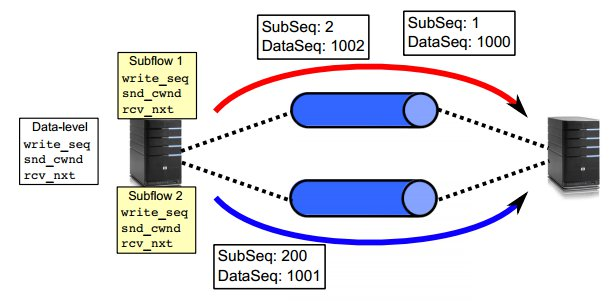
\includegraphics[width=10cm]{dias/Data-Sequence-Mapping.jpg}\\
  \caption{数据序号映射}
\end{figure}
红色子路径上的子路径序号分别是1、2,其数据序号是1000、1002。而下面的蓝色的子路径上的子路径序号和数据序号分别是200,1001。这说明从下面的蓝色子路径已经发送了199个报文,而上面的红色子路径才开始发送。在MPTCP协议定义如下:
\small\begin{verbatim}
                              1                   2                   3
              0 1 2 3 4 5 6 7 8 9 0 1 2 3 4 5 6 7 8 9 0 1 2 3 4 5 6 7 8 9 0 1
             +--------------------------------------------------------------+
             |                Data Sequence Number (8 octets)               |
             +--------------------------------------------------------------+
             |              Subflow Sequence Number (4 octets)              |
             +-------------------------------+------------------------------+
             |  Data-Level Length (2 octets) |        Zeros (2 octets)      |
             +-------------------------------+------------------------------+
\end{verbatim}\normalsize

\subsection{内核的实现}
函数mptcp\_write\_dss\_mapping对 Data Sequeue Number  和  Subflow Sequence Number进行了赋值。实现如下:
\small\begin{verbatim}
"net/mptcp/mptcp_output.c" line 318 of 1667
318 static int mptcp_write_dss_mapping(struct tcp_sock *tp, struct sk_buff *skb,
319                    __be32 *ptr)
320 {
321     struct tcp_skb_cb *tcb = TCP_SKB_CB(skb);
322     __be32 *start = ptr;
323     __u16 data_len;
324
325     *ptr++ = htonl(tcb->seq); /* data_seq */
326
327     /* If it's a non-data DATA_FIN, we set subseq to 0 (draft v7) */
328     if (mptcp_is_data_fin(skb) && skb->len == 0)
329         *ptr++ = 0; /* subseq */
330     else
331         *ptr++ = htonl(tp->write_seq - tp->mptcp->snt_isn); /* subseq */
\end{verbatim}\normalsize
第325行和331行分别对子路径序号和数据序号进行了赋值。
\small\begin{verbatim}
    data_seq and subseq
    The mapping is identify by the relative subflow seq, the data seq and
    the data len. Basically, it means that isn+sub_seq->isn+sub_seq+len at
    the subflow-level corresponds to data_seq->data_seq+len at the
    connection-level.
\end{verbatim}\normalsize
\subsection{数据接收中的重组}
内核使用三种队列接收数据,分别是:Backlog queue(sk$\rightarrow$backlog)、Prequeue queue(tp$\rightarrow$ucopy.prequeue)和 Receive queue (sk$\rightarrow$receeive\_queue)。MPTCP的实现增加了一个新的队列out-of-order queue对于各个子路径收到的数据进行重组。内核中 tcp\_v4\_rcv()的关键实现如下:
\small\begin{verbatim}
"net/ipv4/tcp_ipv4.c" line 1735 of 2581
1735     if (mptcp(tcp_sk(sk))) {
1736         meta_sk = mptcp_meta_sk(sk);
1737
1738         bh_lock_sock_nested(meta_sk);
1739         if (sock_owned_by_user(meta_sk))
1740             skb->sk = sk;
1741     } else {
1742         meta_sk = sk;
1743         bh_lock_sock_nested(sk);
1744     }
1745
1746     ret = 0;
1747     if (!sock_owned_by_user(meta_sk)) {
1748 #ifdef CONFIG_NET_DMA
1749         struct tcp_sock *tp = tcp_sk(meta_sk);
1750         if (!tp->ucopy.dma_chan && tp->ucopy.pinned_list)
1751             tp->ucopy.dma_chan = net_dma_find_channel();
1752         if (tp->ucopy.dma_chan)
1753             ret = tcp_v4_do_rcv(sk, skb);
1754         else
1755 #endif
1756         {
1757             if (!tcp_prequeue(meta_sk, skb))
1758                 ret = tcp_v4_do_rcv(sk, skb);
1759         }
1760     } else if (unlikely(sk_add_backlog(meta_sk, skb,
1761                        meta_sk->sk_rcvbuf + meta_sk->sk_sndbuf))) {
1762         bh_unlock_sock(meta_sk);
1763         NET_INC_STATS_BH(net, LINUX_MIB_TCPBACKLOGDROP);
1764         goto discard_and_relse;
1765     }
1766     bh_unlock_sock(meta_sk);
\end{verbatim}\normalsize
从第1757和1760可以看出skb只进入meta的backlog和prequeue,而和子路径的sock没有什么关系。因此,我们得出包的入队操作如下:
\begin{itemize}
  \item 进入meta\_sk的backlog
  \item 进入meta\_sk的prequeue
  \item 进入子路径的receive\_queue
\end{itemize}
第1和2种入队操作后续操作和正常TCP一致,如果是第3种情况,后续将通过函数mptcp\_queue\_skb()进入tcp\_sk(meta\_sk)$\rightarrow$out\_of\_order\_queue。{\color{red}{我觉得我研究的地方应该是这里}}
\subsection{结论}
\begin{itemize}
  \item MPTCP利用自身的Data Sequeue Number  和  Subflow Sequence Number进行了数据在各种子路径间的传输。此实现独立于TCP。
  \item 为了实现子路径的数据重组,MPTCP利用了队列out\_of\_order\_queue。
\end{itemize}
\newpage
\section{接收端窗口值}
\subsection{简述接收端窗口值}
在TCP协议中影响数据发送的三个因素分别为:发送端窗口值、接收端窗口值和拥塞窗口值。本文主要分析MPTCP中各个子路径对接收端窗口值rcv\_wnd的处理。
\subsection{接收端窗口值的初始化}
根据《MPTCP 源码分析(二) 建立子路径》中描述服务端在发送完SYN/ACK并接收到ACK的时候建立新的sock。在内核实现中,针对连接请求分为两个步骤处理:
\begin{itemize}
  \item SYN队列处理:当服务端收到SYN的时候,此连接请求request\_sock将被存放于listening socket的SYN队列,服务端发送SYN/ACK并等待相应的ACK。
  \item accept队列处理:一旦等待的ACK收到,服务端将会创建新的socket,并将连接请求从listening socket的SYN队列移到其accept队列。
\end{itemize}
当服务端进入LINSTEN状态后,收到第一个SYN包后的处理流程如下:
\begin{figure}[H]
  \centering
  % Requires \usepackage{graphicx}
  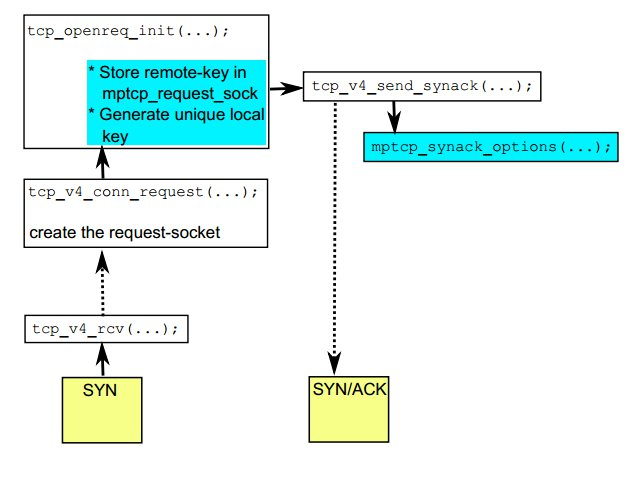
\includegraphics[width=10cm]{dias/Handle-first-SYN.jpg}\\
  \caption{处理第一个SYN包}
\end{figure}
详细的函数调用为:
\small\begin{verbatim}
tcp_v4_rcv
               =》 tcp_v4_do_rcv
                     =》 tcp_rcv_state_process
                         =》mptcp_conn_request
                              =》tcp_v4_conn_request
                                   =》tcp_conn_request
                                        =》tcp_openreq_init
\end{verbatim}\normalsize
在函数tcp\_conn\_request中对连接请求request\_sock进行了分配内存。
\small\begin{verbatim}
"net/ipv4/tcp_input.c" line 6097 of 6195
6097     req = inet_reqsk_alloc(rsk_ops);
6098     if (!req)
6099         goto drop;
\end{verbatim}\normalsize
在函数tcp\_openreq\_init中对request\_sock进行了初始化操作。
\small\begin{verbatim}
1226 static inline void tcp_openreq_init(struct request_sock *req,
1227                     struct tcp_options_received *rx_opt,
1228                     struct sk_buff *skb)
1229 {
1230     struct inet_request_sock *ireq = inet_rsk(req);
1231
1232     req->rcv_wnd = 0;       /* So that tcp_send_synack() knows! */
1233     req->cookie_ts = 0;
1234     tcp_rsk(req)->rcv_isn = TCP_SKB_CB(skb)->seq;
1235     tcp_rsk(req)->rcv_nxt = TCP_SKB_CB(skb)->seq + 1;
1236     tcp_rsk(req)->snt_synack = 0;
1237     req->mss = rx_opt->mss_clamp;
1238     req->ts_recent = rx_opt->saw_tstamp ? rx_opt->rcv_tsval : 0;
1239     ireq->tstamp_ok = rx_opt->tstamp_ok;
1240     ireq->sack_ok = rx_opt->sack_ok;
1241     ireq->snd_wscale = rx_opt->snd_wscale;
1242     ireq->wscale_ok = rx_opt->wscale_ok;
1243     ireq->acked = 0;
1244     ireq->ecn_ok = 0;
1245     ireq->mptcp_rqsk = 0;
1246     ireq->saw_mpc = 0;
1247     ireq->ir_rmt_port = tcp_hdr(skb)->source;
1248     ireq->ir_num = ntohs(tcp_hdr(skb)->dest);
1249 }
\end{verbatim}\normalsize
第1232行对request\_sock的rcv\_wnd进行了初始化为0。

当服务端收到ACK的时候就会建立相应的socket。将会调用tcp\_create\_openreq\_child函数实现,定义如下:
\small\begin{verbatim}
    "include/net/tcp.h" line 578 of 1787
    struct sock *tcp_create_openreq_child(struct sock *sk,
                          struct request_sock *req,
                          struct sk_buff *skb);
\end{verbatim}\normalsize
对于rcv\_wnd的处理具体如下:
\small\begin{verbatim}
"net/ipv4/tcp_minisocks.c" line 441 of 872
512         newtp->window_clamp = req->window_clamp;
513         newtp->rcv_ssthresh = req->rcv_wnd;
514         newtp->rcv_wnd = req->rcv_wnd;
515         newtp->rx_opt.wscale_ok = ireq->wscale_ok;
\end{verbatim}\normalsize
这个阶段为MPTCP的第一条子路径建立情况的三次握手,因此此时创建的socket的属性为master而非slave.

下面的情景为创建一条子路径的情况,当服务端收到第一个SYN包的函数调用情况如下:
\begin{figure}
  \centering
  % Requires \usepackage{graphicx}
  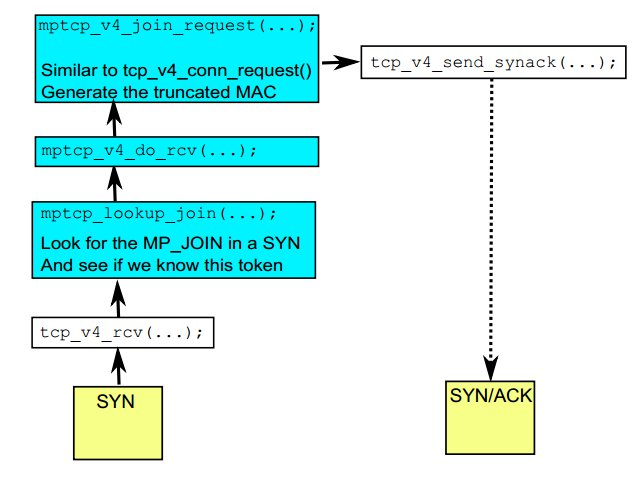
\includegraphics[width=10cm]{dias/Receive-first-SYN.jpg}\\
  \caption{服务端收到第一个SYN包}
\end{figure}
函数mptcp\_v4\_join\_request将会对连接请求request\_sock进行内存分配并初始化。具体的调用如下:
\small\begin{verbatim}
    mptcp_v4_join_request
                           =》tcp_conn_request
                                =》inet_reqsk_alloc
                                =》tcp_openreq_init
\end{verbatim}\normalsize
当客户端的ACK到达后,内核会将此连接请求request\_sock的rcv\_wnd赋值给slave subsocket.
\subsection{master sock 和 slave sock之间接收端窗口值的关系}
TCP在发包的时候会告诉对方自身的接收端窗口值。MPTCP的实现如下:
\small\begin{verbatim}
"net/mptcp/mptcp_output.c" line 992 of 1667
992 u16 mptcp_select_window(struct sock *sk)
993 {
994     u16 new_win     = tcp_select_window(sk);
995     struct tcp_sock *tp = tcp_sk(sk);
996     struct tcp_sock *meta_tp = mptcp_meta_tp(tp);
997
998     meta_tp->rcv_wnd    = tp->rcv_wnd;
999     meta_tp->rcv_wup    = meta_tp->rcv_nxt;
1000
1001     return new_win;
1002 }
\end{verbatim}\normalsize
第994获得最新的窗口值并返回。第998行将slave sock的rcv\_wnd赋值给master sock。

第994行的函数tcp\_select\_window的实现如下:
\small\begin{verbatim}
"net/ipv4/tcp_output.c" line 275 of 3327
275 u16 tcp_select_window(struct sock *sk)
276 {
277     struct tcp_sock *tp = tcp_sk(sk);
278     /* The window must never shrink at the meta-level. At the subflow we
279      * have to allow this. Otherwise we may announce a window too large
280      * for the current meta-level sk_rcvbuf.
281      */
282     u32 cur_win = tcp_receive_window(mptcp(tp) ? tcp_sk(mptcp_meta_sk(sk)) : tp);
283     u32 new_win = tp->__select_window(sk);
\end{verbatim}\normalsize
对于第283行的\_\_select\_window()函数,MPTCP的内核实现如下:
\small\begin{verbatim}
"net/mptcp/mptcp_output.c" line 771 of 1667
771 u32 __mptcp_select_window(struct sock *sk)
772 {
773     struct inet_connection_sock *icsk = inet_csk(sk);
774     struct tcp_sock *tp = tcp_sk(sk), *meta_tp = mptcp_meta_tp(tp);
775     struct sock *meta_sk = mptcp_meta_sk(sk);
776     int mss, free_space, full_space, window;
777
778     /* MSS for the peer's data.  Previous versions used mss_clamp
779      * here.  I don't know if the value based on our guesses
780      * of peer's MSS is better for the performance.  It's more correct
781      * but may be worse for the performance because of rcv_mss
782      * fluctuations.  --SAW  1998/11/1
783      */
784     mss = icsk->icsk_ack.rcv_mss;
785     free_space = tcp_space(meta_sk);
786     full_space = min_t(int, meta_tp->window_clamp,
787             tcp_full_space(meta_sk));
788
789     if (mss > full_space)
790         mss = full_space;
791
792     if (free_space < (full_space >> 1)) {
793         icsk->icsk_ack.quick = 0;
794
795         if (tcp_memory_pressure)
796             /* TODO this has to be adapted when we support different
797              * MSS's among the subflows.
798              */
799             meta_tp->rcv_ssthresh = min(meta_tp->rcv_ssthresh,
800                             4U * meta_tp->advmss);
801
802         if (free_space < mss)
803             return 0;
804     }
805
806     if (free_space > meta_tp->rcv_ssthresh)
807         free_space = meta_tp->rcv_ssthresh;
808
809     /* Don't do rounding if we are using window scaling, since the
810      * scaled window will not line up with the MSS boundary anyway.
811      */
812     window = meta_tp->rcv_wnd;
813     if (tp->rx_opt.rcv_wscale) {
814         window = free_space;
815
816         /* Advertise enough space so that it won't get scaled away.
817          * Import case: prevent zero window announcement if
818          * 1<<rcv_wscale > mss.
819          */
820         if (((window >> tp->rx_opt.rcv_wscale) << tp->
821              rx_opt.rcv_wscale) != window)
822             window = (((window >> tp->rx_opt.rcv_wscale) + 1)
823                   << tp->rx_opt.rcv_wscale);
824     } else {
825         /* Get the largest window that is a nice multiple of mss.
826          * Window clamp already applied above.
827          * If our current window offering is within 1 mss of the
828          * free space we just keep it. This prevents the divide
829          * and multiply from happening most of the time.
830          * We also don't do any window rounding when the free space
831          * is too small.
832          */
833         if (window <= free_space - mss || window > free_space)
834             window = (free_space / mss) * mss;
835         else if (mss == full_space &&
836              free_space > window + (full_space >> 1))
837             window = free_space;
838     }
839
840     return window;
841 }
\end{verbatim}\normalsize
影响window的计算的因素为:
\begin{itemize}
  \item 收到的MSS( icsk$\rightarrow$icsk\_ack.rcv\_mss)
  \item 套接字缓冲区总的空间(tcp\_full\_space)
  \item 套接字缓冲区的空闲空间(tcp\_space)
  \item meta\_tp$\rightarrow$rcv\_ssthresh  /* Current window clamp */
\end{itemize}
观察上面的代码可以知道MPTCP的实现和\_\_tcp\_select\_window的区别是都是依据meta\_tp,而非tp。这说明master sock 和 其余slave sock使用相同的 rcv\_wnd。
\subsection{结论}
\begin{itemize}
  \item master sock 和 其余slave sock使用相同的接收缓冲区和 rcv\_wnd。
\end{itemize}
\newpage
\section{数据重发}
\subsection{简述数据重发}
TCP使用定时器函数tcp\_retransmit\_timer进行数据重发,MPTCP需要重发数据的时候,不仅仅在原路径发送数据,而且会在另外一条子路径进行重发。这样考虑的原因是:考虑网络中间件设备的影响, 保证子路径上数据序列号的完整性。目前的版本0.89依然如此实现,以后应该会优化。
\subsection{内核实现}
MPTCP的结构如下图所示:
\begin{figure}[H]
  \centering
  % Requires \usepackage{graphicx}
  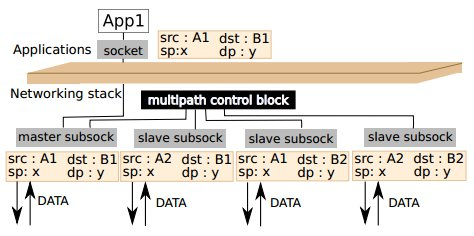
\includegraphics[width=10cm]{dias/Kernal.jpg}\\
  \caption{MPTCP的结构图}
\end{figure}
如上图所示:每一个slave subsock 和 master subsock实际上维持着一个正常的TCP链路,因此,他们都具有重发定时器tcp\_write\_timer。MPTCP实现的思路就是:每个子链路发送失败的时候,将发送失败的SKB拷贝一份到meta sock。然后让meta sock 再次选择另外一条子路径发送。

如下是对tcp\_retransmit\_timer的修改:
\small\begin{verbatim}
"net/ipv4/tcp_timer.c"  line 488 of 691
487
488 out:;
489     if (mptcp(tp)) {
490         mptcp_reinject_data(sk, 1);
491         mptcp_set_rto(sk);
492     }
493 }
\end{verbatim}\normalsize
函数mptcp\_reinject\_data的实现如下:
\small\begin{verbatim}
"net/mptcp/mptcp_output.c" line 237 of 1667
236 /* Inserts data into the reinject queue */
237 void mptcp_reinject_data(struct sock *sk, int clone_it)
238 {
239     struct sk_buff *skb_it, *tmp;
240     struct tcp_sock *tp = tcp_sk(sk);
241     struct sock *meta_sk = tp->meta_sk;
242
243     /* It has already been closed - there is really no point in reinjecting */
244     if (meta_sk->sk_state == TCP_CLOSE)
245         return;
246
247     skb_queue_walk_safe(&sk->sk_write_queue, skb_it, tmp) {
248         struct tcp_skb_cb *tcb = TCP_SKB_CB(skb_it);
249         /* Subflow syn's and fin's are not reinjected.
250          *
251          * As well as empty subflow-fins with a data-fin.
252          * They are reinjected below (without the subflow-fin-flag)
253          */
254         if (tcb->tcp_flags & TCPHDR_SYN ||
255             (tcb->tcp_flags & TCPHDR_FIN && !mptcp_is_data_fin(skb_it)) ||
256             (tcb->tcp_flags & TCPHDR_FIN && mptcp_is_data_fin(skb_it) && !skb_it->len))
257             continue;
258
259         __mptcp_reinject_data(skb_it, meta_sk, sk, clone_it);
260     }
261
262     skb_it = tcp_write_queue_tail(meta_sk);
263     /* If sk has sent the empty data-fin, we have to reinject it too. */
264     if (skb_it && mptcp_is_data_fin(skb_it) && skb_it->len == 0 &&
265         TCP_SKB_CB(skb_it)->path_mask & mptcp_pi_to_flag(tp->mptcp->path_index)) {
266         __mptcp_reinject_data(skb_it, meta_sk, NULL, 1);
267     }
268
269     mptcp_push_pending_frames(meta_sk);
270
271     tp->pf = 1;
272 }
\end{verbatim}\normalsize
第259行的\_\_mptcp\_reinject\_data函数将出现超时的sk$\rightarrow$sk\_write\_queue的数据拷贝到 meta\_sk 的reinject queue。\\
而269行的函数mptcp\_push\_pending\_frames将会对reinject queue中的数据进行发送,其调用关系如下:
\small\begin{verbatim}
    mptcp_push_pending_frames
                            =》__tcp_push_pending_frames
                                 =》tcp_sk(sk)->write_xmit
                                      =》mptcp_write_xmit
                                           =》mptcp_next_segment
                                                =》__mptcp_next_segment
                                                =》get_available_subflow
\end{verbatim}\normalsize
\subsection{结论}
\begin{itemize}
  \item 子路径出现重发数据的情况下,MPTCP会选择另外一条路径发送同样的数据。
\end{itemize}
\newpage
\section{拥塞控制}
\subsection{简述拥塞控制}
MPTCP的拥塞控制对TCP的拥塞控制的线性增加阶段进行了修改,而慢启动,快速重传、快速恢复都没有改变。每条子路径拥有自己的cwnd,MPTCP的拥塞算法主要关心cwnd的改变。
\subsection{拥塞算法设计原则}
\begin{itemize}
  \item MPTCP的Throughput 要达到MPTCP中所有子路径中最好的一条路径
  \item MPTCP应该和普通TCP一样从共享资源中获得相同资源
  \item MPTCP中的流量将从拥塞的子路径转移到不拥塞的路径。
\end{itemize}
\subsection{算法理解}
MPTCP的各个子路径运行着正常的TCP,因此直观的我们可以在每条子路径上运行自己的拥塞控制算法,但是这样就违背了设计原则2,这样的效果是MPTCP的吞吐量就会超过其他正常TCP。因此有如下EWTCP算法(n表示路径数量,$a=\frac{1}{\sqrt{n}}$):
\begin{description}
  \item[对于路径r上的每一个ACK] 窗口增加的数值$W_r=\frac{a}{W_r}$
  \item[对于路径r上的每一个LOSS] 窗口减少的数值$W_r=\frac{W_r}{2}$
\end{description}
a的取值参考~\cite{Honda2009Multipath},这样,MPTCP就把每次cwnd的增加分摊到各个不同的子路径上,这样MPTCP就和正常TCP有着相同的吞吐量。但是这样的算法设计存在问题,不能有效的利用网络环境,我们应该根据设计原则3,将流量移动到拥塞情况最少的路径上去。因此有如下COUPLED算法($W_t$是所有子流的窗口之和):
\begin{description}
  \item[对于路径r上的每一个ACK] 窗口增加的数值$W_r=\frac{1}{W_t}$
  \item[对于路径r上的每一个LOSS] 窗口减少的数值$W_r=\frac{W_t}{2}$
\end{description}
此算法让各个子路径的拥塞窗口的变化联系起来,比如有两条路径,一条路径上面拥塞导致导致丢包严重,那么不断的减少$W_t/2$,这样的话,就将流量从拥塞的路径移动到不拥塞的路径上。但是,这个算法存在两个问题:
\begin{itemize}
  \item 如果拥塞的子路径完全没有流量,我们就无从得知这条子路径上拥塞情况以后是不是会改善。
  \item 没有考虑到RTT的的因素,比如对于一个智能手机来说,3G网络和WIFI相比丢包率更低,而RTT更大。
\end{itemize}
但是因为3G的拥塞情况更好,因此流量大部分会通过3G网络。而3G网络的吞吐量可能小于WIFI的吞吐量。因此提出MPTCP的拥塞控制算法($W_r$的路径r的当前窗口值):
\begin{description}
  \item[对于路径r上的每一个ACK] 窗口增加的数值$W_r=\min(\frac{a}{W_t},\frac{1}{W_r})$
  \item[对于路径r上的每一个LOSS] 窗口减少的数值$W_r=\frac{W_r}{2}$
\end{description}
此算法通过 min操作来遵守设计原则2,通过a来保证各个子路径上都有适当的流量,从而达到设计原则1和3,详细的算法描述可以参考~\cite{Wischik2011Design}。
\subsection{MPTCP的内核实现}
MPTCP会在接收每一个ACK的时候,计算算法中的a。调用情况如下:
\small\begin{verbatim}
     tcp_ack()
               =>tcp_ca_event()
                    =>cwnd_event()
                         =>mptcp_ccc_cwnd_event()
\end{verbatim}\normalsize

在tcp\_ack函数中也会增加cwnd,调用情况如下:
\small\begin{verbatim}
     tcp_ack()
               =>tcp_cong_avoid()
                    =>cong_avoid()
                         => mptcp_ccc_cong_avoid()
\end{verbatim}\normalsize


\bibliographystyle{unsrt}
\bibliography{Referenzarchiv}

\end{document}

